\chapter{Klassen}

In diesem Kapitel geht es in erster Linie darum zu erklären, was Klassen sind und wie sie (programmtechnisch) Verwendung finden. Ihre Herkunft und den theoretischen Hintergrund von Klassen im Abstraktionsmechanismus der objektorientierten Programmierung werden wir in Kapitel \ref{chap:oop} kennen lernen.

\section{Objekte und Instanzen}

\subsection{Was ist eine Instanz?}\label{ref:instance}\index{Instanz}

Ein Begriff, welcher dem der Instanz am nächsten kommt, ist "'temporäres Exemplar"'.\index{Exemplar, temporär} In der Biologie sind Exemplare – wie z.B. Eichhörnchen oder Pusteblumen – einzelne Lebewesen. Sie können über die Klasse der Säugetiere reden, aber wenn Sie einen Löwen vor sich sehen, sollten Sie über dieses spezielle Exemplar nachdenken (als gut gemeinter Rat). Das selbe gilt für die informationstechnischen Exemplare. Und als temporär sind diese Exemplare zu verstehen, weil sie eine strikt begrenzte „Lebensdauer“\index{Lebensdauer} haben. Den Begriff Lebensdauer möchte ich nicht formal definieren. Ich glaube, es ist klar, was damit gemeint ist, solange von biologischen Exemplaren die Rede ist. Informationstechnische Exemplare haben ebenfalls etwas das als Lebensdauer verstanden werden kann, nämlich die Zeitspanne zwischen ihrer Erzeugung, d.h. der Zuweisung eines bestimmten Bereichs des Hauptspeichers eines Computers bis zur Zerstörung, d.h. Freigabe des Hauptspeichers der diesem Exemplar zugewiesen war. Als Hinweis, Instanzen können noch in sogenannten „serialisierten“ Zuständen ihre Lebensdauer in einem persistenten Zustand fristen. Dies wird später noch genauer erklärt. 

Exemplare sind spezielle, existierende Dinge, die klassifiziert werden können. An dieser Stelle sollten Sie sich nicht zu sehr an den Begriff Klasse orientieren, denn der wird später noch erklärt. Zwar sind Objekte Instanzen von Klassen, aber der Instanz Begriff sollte hier weiter gefasst verstanden werden. Denn Klassen können ihrerseits wieder Instanzen von anderen Dingen sein, sogenannten Meta-Klassen. Und wenn Sie Computer-Rollen-Spiele kennen, werden Ihnen „Instanzen“ als spezielle Teile eines Dungeons untergekommen sein, die ihrerseits wiederum Instanzen einer abstrakten Dungeon Beschreibung sind. Das vorletzte Vorkommen von Instanz habe ich in Anführungsstriche geschrieben, da die Hersteller von Computer-Rollen-Spielen vermutlich eine eigene Definition vom Begriff Instanz haben. In der hier hergestellten Interpretation des Begriffs passt die temporäre, für eine Gruppe von Spielern hergestellte Kopie eines Dungeons aber recht gut. Fassen wir hier in einer Auflistung kurz die wesentlichen Eigenschaften einer Instanz zusammen: 

\begin{enumerate}
\item Eine Instanz ist klassifizierbar -- in welcher Weise dies geschieht ist nicht definiert!
\item Sie ist ein „real“ existierendes Exemplar -- sofern der Begriff real auf Objekte im Hauptspeicher eines Computers angewendet werden kann.
\item Ihre Existenz ist zeitlich begrenzt
\end{enumerate}


\subsection{Was ist ein Objekt?}\index{Objekt}

Im Grunde reden Sie bei einem Objekt immer von einer Instanz. Diese Begriffe sollten synonym verwendet werden. Warum ich hier einen eigenen Abschnitt für Objekte einfüge und nicht einfach bei Instanzen die Bemerkung fallen lasse, dass Objekte Instanzen sind, liegt darin begründet, dass die Verwendung des Begriffs Objekt oft sehr schwammig ist. Viele Programmierer werfen mit Floskeln um sich wie z.B. „alles ist ein Objekt“. Aber auch der Begriff „Objektorientierte-Programmierung“ ist schon so ungenau in seiner Verwendung, dass die ursprüngliche Definition kaum noch darin auszumachen ist. 

Konsequent lautet die ISO Definition des Begriffs "`objektorientiert"' (siehe \cite{isooo}):\index{objektorientiert}

\begin{quote}
Bezieht sich auf eine Technik oder Programmiersprache, welche Objekte, Klassen und Vererbung unterstützt.
\end{quote}

Na prima. Dem entgegen stehen objektorientierte Sprachen, die keine Klassen brauchen (Prototypenbasierte Programmierung; JavaScript) sowie der Umstand, dass dem Vererbungsbegriff heute nicht mehr die Bedeutung zu kommt, wie noch am Anfang der Euphorie. 

Abgesehen von dem ganzen Durcheinander, das mit den Begriffen "`objektorientiert"' und "`Objekt"' angestellt wurde, reicht es für uns zu wissen, dass ein Objekt (oder eine Instanz) ein Ding ist, das sich im Hauptspeicher unseres Rechners (genauer gesagt des virtuellen Rechners JVM) befindet und unter einem Namen angesprochen werden kann. Dieser Name ist eine sogenannte Referenz (englisch Pointer), der auf einen Bereich des Hauptspeichers verweist. 

\section{Klassen}\index{Klasse}

Eine Klasse ist zunächst einmal nicht mehr als ein Name mit einer öffnenden und einer schließenden, geschweiften Klammer. Die Minimale Klasse, die man definieren kann ist:
\begin{lstlisting}
class Person {
}
\end{lstlisting}
Des Weiteren können Klassen Variablen Definitionen enthalten -- bei Klassen heißen diese dann "`Member"', sowie Funktionen, die innerhalb der Klasse definiert werden. Beispiel:\index{Member}
\begin{figure}[h]
\begin{lstlisting}
class Person {
  private int age;

  public int getAge() {
    return age;
  }
  
  public void setAge(int value) {
    age = value;
  }
}
\end{lstlisting}
\caption{Eine sehr einfache Klasse}
\label{code:class}
\end{figure}

Ok, hier haben wir schon einige Dinge gleichzeitig gemacht, die ich der Reihenfolge nach erklären möchte.

\subsection{Member}\index{Member}
Gehen wir einen Schritt zurück und überlegen, was mit dem Begriff "`Variable"' gemeint ist. Variablen sind Namen für (noch) nicht bekannte Werte. Genauso, wie wir sie bei der Definition der komplexen Zahlen verwendet haben in der Einleitung in Formel (\ref{eq:komplex}). Dort haben wir die Variablen $a$ und $b$ als reelle Zahlen definiert, deren Wert völlig unbestimmt ist. Wir wissen lediglich welcher "`Art"' oder welchen Typs diese Variablen sind. Dies ist Teil des sogenannten Typ-Konzept von Java. Jeder Variable muss ein sogenannter Typ zugewiesen sein, damit Java mit ihnen umgehen kann. Dies dient zum einen dazu, damit immer ausreichend Speicher für die Werte einer Variable beantragt werden kann, sowie auch zu Ihrer eigenen Sicherheit, dass Sie wissen, was Sie mit einer Variablen tun können. Es ist zum Beispiel unsinnig einen ganzzahligen Wert zu einer Zeichenkette hinzu zu summieren und zu erwarten, dass eine Fließkommazahl dabei heraus kommt, darüber beschwert sich dann der Java Compiler (zu recht) in Abbildung \ref{nb:typeerror}.

\begin{figure}[h]
\centering
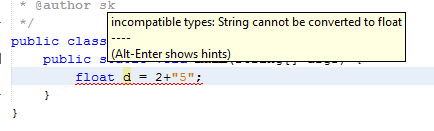
\includegraphics[]{img/nb004}
\caption{Typ Fehler im Netbeans Editor}
\label{nb:typeerror}
\end{figure}

Netbeans beschwert sich, dass die Zeichenkette (in englisch String) nicht zu einem "`float"' konvertiert werden kann. Diese Fehlermeldung sagt uns zwei Dinge. Zum einen, dass man nicht einfach so einen String zu einem Zahlenwert machen kann, auch wenn wir der Anschauung nach glauben, die 5 in den Anführungsstrichen sei ja nichts anderes als eine Zahl. Und zum zweiten, dass die ganze Zahl 2 sehr wohl automatisch zu einer Fließkommazahl konvertiert werden kann. Auf dieses Thema werden wir noch in Kapitel \ref{ref:conversion} zurück kommen.

\subsubsection{Primitive Datentypen}\index{Primitive}\index{primitive Datentypen}
In Java gibt es folgende primitive (d.h. nicht als Klasse dargestellte) Datentypen:

\begin{description}
\item[boolean] 1 Bit, true/false
\item[byte] 8 Bit
\item[char] x Bit, kann ein UTF-8 Charakter sein und somit von nicht vorherbestimmter Länge.
\item[short] 16 Bit, kurzer Ganzzahlwert
\item[int] 32 Bit langer Ganzzahlwert
\item[long] 64 Bit langer Ganzzahlwert
\item[float] 32 Bit langer Fließkommawert im IEEE 754 Standard
\item[double] 64 Bit langer Fließkommawert im IEEE 754 Standard
\end{description}

Ganzzahlwerte sind suggestiver weise Zahlen, die keine Nachkommastellen besitzen. Fließkommawerte sollten vielleicht etwas näher erklärt werden, denn sie sind nicht einfach Zahlen mit Nachkommastellen. Der Wert einer Fließkommazahl ist auf den Bereich zwischen +10 und -10 "`normiert"'. Das bedeutet, jede beliebige Dezimalzahl wird so dargestellt, dass man sie solange mit 10 multipliziert oder durch 10 dividiert, bis sich eine Zahl zwischen +10 und -10 ergibt. Die Anzahl der Multiplikationen oder Divisionen mit 10 merkt man sich in einer zweiten Zahl. Die normierte Zahl zwischen -10 und +10 wird "`Mantisse"' genannt, während die Anzahl der Multiplikationen oder Divisionen "`Exponent"' genannt wird. Diese Darstellung wird auch oft als Ingenieursdarstellung bezeichnet. Beispiel:\index{Fließkommawert}\index{Ganzzahlwert}
\begin{equation*}
1.03888E-12 = 1.03888\cdot 10^{-12} = 0.00000000000103888
\end{equation*}

Der IEEE\footnote{\textbf{Institue of Electrical and Electronics Engineers}\index{IEEE}, meistens als "`I tripple E"' bezeichnet.} 754 Standard bestimmt für 32 Bit Werte eine 23 Bit lange Mantisse sowie einen 7 Bit langen Exponenten und für 64 Bit Werte eine 52 Bit lange Mantisse sowie einen 10 Bit langen Exponenten. Jeweils ein Vorzeichen Bit für Mantisse und Exponenten müssen hinzugerechnet werden.

Für alle oben dargestellten primitiven Datentypen gibt es sogenannte Wrapper Klassen, wie in Tabelle \ref{tab:wrapper} aufgeführt.

\begin{table}[h]
\centering
\begin{tabular}{r|l}
\hline
Primitiv & Wrapper \\
\hline
boolean & Boolean \\
byte & Byte \\
char & Character \\
float & Float \\
int & Integer \\
long & Long \\
short & Short \\
double & Double \\
\hline
\end{tabular}\\[3mm]
\caption{Wrapper Klassen der primitiven Datentypen} \label{tab:wrapper}
\end{table}

Wie Sie sehen, brauchen Sie für die Nutzung der Wrapper (abgesehen von char und int) lediglich den ersten Buchstaben zu ändern. Die Typen char und int wurden (vermutlich) deswegen nicht character und integer genannt, weil in der Programmiersprache C diese Datentypen auch char und int heißen. Und da die Syntax von Java sich an C und C++ orientiert, blieb es wohl dabei.

\subsection{Funktion}\index{Funktion}
Klassen stellen eine Kombination von Daten und Funktionalität dar. Wobei es sinnvoll ist, die Funktionalität nicht von den Daten zu trennen, sondern sie im Gegenteil daraufhin abzustimmen. Klingt etwas kompliziert, ist aber ein relativ einfacher Vorgang. Nämlich anstatt dass auf die Variablen einer Klasse jeder Zugriff hat, versteckt man sie. Dies geschieht mit dem Zusatz "`private"' an der Variablen. Auf eine als privat deklarierte Variable kann von keinem anderen Code zugegriffen werden, als von der Klasse selbst, zu der die Variable gehört. Mehr dazu im Kapitel \ref{chap:encapsule}. Sie ist somit ein exklusives Mitglied (Member) einer Klasse. Und sie stellt in einem gewissen Sinn den Status dar, welcher nur über die Zugriffs-Funktionen verändert werden kann. In unserem Beispiel die \texttt{getAge()} und \texttt{setAge()} Funktionen der Klasse in Abbildung \ref{code:class}. 

Auf diese Zugriffsfunktionen (oder Methoden) beschränkt sich natürlich nicht das Spektrum der Funktionen. In diesen Funktionen wird die eigentliche Arbeit erledigt, für die man Programme im allgemeinen benutzt. Daher lohnt es sich, diese etwas genauer anzusehen:

Funktionen bestehen aus vier Teilen: Einem Namen, unter dem sie angesprochen werden, einer Liste von sogenannten Parametern, einem Rückgabewert und einer Implementierung. Eine Funktion wird immer so aussehen:
\begin{lstlisting}
<Typ> name(Typ parameter1, Typ parameter2, Typ parameter3) {
}
\end{lstlisting}




\section{Instanziierung}\index{Instanziierung}

Wir hatten in Abschnitt \ref{ref:instance} gelernt, was eine Instanz ist. Und dabei definiert, dass Instanzen in einem gewissen Sinne klassifizierbar sind. Dies wollen wir hier nun konkretisieren. Im vorherigen Abschnitt haben wir erklärt, was eine Klasse ist. Doch sind Klassen keine temporäre Exemplare, wie wir dies für Instanzen festgestellt hatten. Klassen sind eher Schablonen, anhand derer ihre temporären Exemplare (oder halt eben Instanzen) hergestellt werden können. Für die Instanzen wird dann vom Runtime Environment Speicher besorgt und zugewiesen. Und zwar genau so viel, wie die Klasse definiert hatte. In diesem Speicher legt die Instanz die Werte ihrer Variablen ab. In unserem Beispiel wäre das nur ein Integer für das Alter einer Person. Die Erzeugung einer Instanz anhand einer Klassen-Schablone wird Instanziierung genannt.\index{Instanziierung}

Wie sagt man nun der Virtual Machine, dass man Speicher für eine bestimmte Instanz haben möchte? Dies geschieht mit dem sogenannten "`new"'-Operator.\index{new}\index{new Operator} Der new-Operator fragt nach Speicher und weist diesen, in der zur Klasse passenden Größe, einer Variablen zu, z.B.:
\begin{lstlisting}
Person p = new Person();
\end{lstlisting}
Unter dem Namen "`p"' können wir ab diesem Moment auf diese spezielle Instanz zugreifen.

Klassen sind also die Beschreibungen der inneren Struktur von Instanzen. Man sagt demnach auch ein bestimmtes Objekt sei die Instanz einer bestimmten Klasse. 

Es ist wichtig zu verstehen, dass die verschiedenen Instanzen einer Klasse sich den Code der Klassen-Funktionen teilen. Also nicht jedes Objekt hat seine eigenen \texttt{getAge()} und \texttt{setAge()} Funktionen. Alle Objekte teilen sich diese "`Implementierung"'. Ändert man die Implementierung, ändert sich das Verhalten aller Objekt dieser Klasse. Das gilt wiederum nicht für die Variablen. Jedes Objekt hat seine eigene Kopie der von der Klasse definierten Variablen. 

\noindent Erweiterten wir die Person-Klasse aus unserem Beispiel:

\begin{lstlisting}
class Person {
    private String firstName;
    private String lastName;
    private int age;

    public String getFirstName() {
        return firstName;
    }

    public void setFirstName(String firstName) {
        this.firstName = firstName;
    }

    public String getLastName() {
        return lastName;
    }

    public void setLastName(String lastName) {
        this.lastName = lastName;
    }

    public int getAge() {
        return age;
    }

    public void setAge(int age) {
        this.age = age;
    }
}
\end{lstlisting}



Wir haben eine Klasse, die Personen definiert. Jede Person hat demnach einen Vor-, Nachnamen und ein Alter. Dies stellt sozusagen die Basis dar, die alle als Person klassifizierte Objekte gemeinsam haben. Sehen wir uns ein spezielles Exemplar an: Heinz Meier, 69.

\begin{lstlisting}
Person p = new Person();
p.setFirstName("Heinz");
p.setLastName("Meier");
p.setAge(69);
\end{lstlisting}

\subsection{Konstruktor}\index{Konstruktor}

Hinter dem new-Operator steht etwas das, aufgrund der Klammern, aussieht wie eine Funktion. Dies ist auch eine Funktion, der sogenannte Konstruktor. Der Konstruktor ist eine spezielle Funktion, die nur bei der Erzeugung einer Instanz aufgerufen wird und üblicherweise der Initialisierung der Instanz dient. Klassen müssen mindestens einen Konstruktor haben, können aber mehrere besitzen. Wer genau aufgepasst hat, wird feststellen, dass in unserer Person Klasse kein Konstruktor mit dem Namen "`Person()"' definiert worden war (oder irgendein anderer Konstruktor).

Wenn der Java Compiler keinen Konstruktor findet, erzeugt er automatisch den sogenannten "`Default-Konstruktor"'.\index{Default-Konstruktor} Der Default-Konstruktor besitzt keinen Parameter und per Definition besitzt kein Konstruktor einen Rückgabewert. In unserem Beispiel hätte er also die folgende Form:
\begin{lstlisting}
public Person() {
}
\end{lstlisting}
Der Default-Konstruktor ist per Definition immer public deklariert, das bedeutet, jeder kann ihn verwenden. Wenn es einen Konstruktor gibt, erzeugt der Compiler \textbf{keinen} Default-Konstruktor. Das kann zu der verwirrenden Situation führen, dass die Erzeugung einer Instanz vor einer Änderung noch funktionierte, danach aber nicht mehr, weil man einen ganz andersartigen Konstruktor der Klasse hinzufügte. Existieren Konstruktoren und man braucht den Default-Konstruktor, muss man ihn manuell hinzufügen. 

Konstruktoren werden oft dazu verwendet, die Benutzung der Klasse zu bestimmen. Hätten wir zum Beispiel die Vorstellung, dass es nicht möglich sein sollte, eine Person Instanz zu erzeugen, die keinen Namen besitzt, so könnten wir dies vorgeben, indem wir den Konstruktor hinzufügen:
\begin{lstlisting}
public Person(String fName, String lName) {
  firstName = fName;
  lastName = lName;
}
\end{lstlisting}
Dies würde dazu führen, dass der Compiler keinen Default-Konstruktor mehr erzeugt und der Aufruf 
\begin{lstlisting}
Person p = new Person();
\end{lstlisting}
nicht kompilierbar ist. Dagegen
\begin{lstlisting}
Person p = new Person("Heinz", "Meier");
\end{lstlisting}
aber schon. Und das hat den zusätzlichen Effekt, dass Vor- und Nachname unserer Person Instanz bereits gesetzt ist.

\subsection{Getter und Setter}\label{chap:getset}\index{Getter}\index{Setter}

In Java gibt es das sogenannte "`Bohnen"'\index{Java Beans} (Java Beans)\footnote{Aufgrund dessen, dass Java nach einer Kaffee Sorte benannt wurde, die von den Entwicklern gerne und in Mengen verkonsumiert wurde, sind diese Bohnen oft als Kaffee-Bohnen dargestellt.}. Dies sind Klassen, die einigen Vorgaben genügen. Wir kennen noch nicht genug von der Java-Sprache, dass wir alle Vorgaben verstehen würden, doch eine Vorgabe haben wir mit unserer Person Klasse bereits erfüllt, nämlich dass auf interne Variablen nur über Funktionen zugegriffen werden darf, deren Namen einem bestimmten Schema folgen. Diese Funktionen nennt man die Getter und Setter einer Variable in Anlehnung an die englischen Verben "`to get"' und "`to set"'.

Für eine Variable müssen die Setter und Getter in der folgenden Art erzeugt werden:

\begin{enumerate}
\item Der Getter muss mit "`get"' beginnen. Ist der Variablen Wert boolean oder Boolean, muss sie mit "`is"' beginnen.
\item Der Name des Getters wird erweitert um den Namen der Variable. Der erste Buchstabe der Variablen wird zu einem Großbuchstaben, wenn er das nicht schon war.
\item Der Getter muss einen Rückgabetyp haben, der identisch ist mit dem Typ der Variablen.
\item Der Setter muss mit "`set"' beginnen. Auch für boolean Variablen.
\item Der Setter Name wird um den Variablen Namen erweitert, wie der Getter. 
\item Der Setter muss einen Parameter vom identischen Typ wie die Variable besitzen. 
\end{enumerate}
Diese Vorgehensweise ist so streng vorgegeben, dass die IDE's diese Funktionen automatisch erzeugen können. Probieren wir das einmal aus. Erzeugen Sie in Netbeans eine Person Klasse, die nur die privaten Variablen besitzt:

\begin{lstlisting}
public class Person {
  private String firstName;
  private String lastName;
  private int age;
}
\end{lstlisting}
Klicken Sie nun mit der rechten Maustaste irgendwo zwischen den geschweiften Klammern und wählen Sie aus dem (zugegebenermaßen unhandlich gro\-ßen) Kontextmenü den Punkt "`Insert Code ..."'. Alternativ können Sie die Tasten "`Alt"'+"'Einfg"' drücken. Danach erscheint ein kleineres Kontextmenü, wählen Sie dort "`Getter and Setter..."' aus. In dem folgenden Dialog können Sie die Variablen auswählen, für die Sie die Getter und Setter erzeugen möchten. Wählen Sie alle aus, wie in Abbildung \ref{nb:getset}
\begin{figure}[h]
\centering
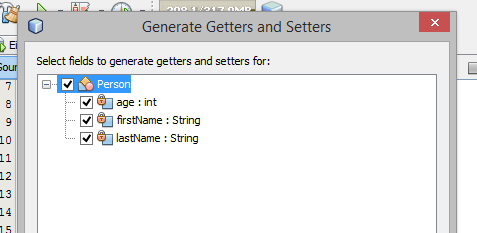
\includegraphics[width=\textwidth]{img/nb005}
\caption{Auswahl der Variablen für die Getter und Setter erzeugt werden sollen}
\label{nb:getset}
\end{figure}
und klicken Sie dann auf "`generate"'. Daraufhin erzeugt die IDE die Getter und Setter. Dies funktioniert in allen IDE's, lediglich der Ort, wo man den Generator findet, ist zuweilen verschieden. 

Mit dem Schreiben solcher Getter und Setter sollte man sich nicht mehr aufhalten. Lassen Sie die IDE dies erledigen. Dann kommen Sie auch nicht in Versuchung, aufgrund von Schreibfaulheit gegen die vorher genannten Regeln zu verstoßen.


\section{Typensystem}\index{Typ}\index{Typisierung}

Java ist eine streng typisierte Sprache (manchmal auch als stark typisiert bezeichnet). Die Definition dieses Begriffs ist leider nicht eindeutig, daher müssen wir ihn hier für uns definieren:

In einer streng typisierten Sprache:
\begin{enumerate}
\item muss jede Variable ei\-nen eindeutigen Typ besitzen,
\item sind Konvertierung von Variablen verschiedener Typen nur in sehr begrenztem, von der Sprache selbst definiertem, Umfang möglich,
\item muss die Typ-Überprüfung zum Zeitpunkt des Kompilierens durchgeführt werden.
\end{enumerate}

Diese Definition mag für manchen entweder nicht ausreichend, oder zu streng sein. Darüber kann man diskutieren. Für die Zwecke in diesem Buch möchte ich die Typisierung in dieser Form definieren, denn sie wird zum einen erklären, warum wir nicht deklarierte Variablen nicht verwenden dürfen. Und zum anderen, warum wir beliebige Objekte nicht in andere Objekte umwandeln können.

\subsection{Konvertierung}\label{ref:conversion}\index{Konvertierung}
Die Konvertierung einer Variablen des einen Typs in einen anderen Typ ist nur für die primitiven Datentypen eine "`einfache"' Sache. Bei komplexen Objekten ist sie praktisch unmöglich und nur dann zulässig, wenn strenge Verwandschaftsbeziehungen zwischen den Typen, zwischen denen konvertiert werden soll, existieren. Siehe Kapitel \ref{chap:inherit} zum Thema Vererbung.

Sehen wir uns an einem Beispiel genauer an, worum es geht. 


\subsection{Autoboxing und Unboxing}\label{ref:autoboxing}\index{Autoboxing}\index{Unboxing}
TODO


\section{Generics}\index{Generics}
TODO

\section{Unser Projekt}

Für das in der Einleitung beschriebene Projekt brauchen wir (unter vielen anderen Dingen) eine Möglichkeit, mit komplexen Zahlen zu rechnen. Wir könnten natürlich immer mit zwei reellen Zahlen arbeiten, bzw. ihren endlichen Entsprechungen in einem Computer: "`float"' oder "`double"'. 

Aber wir möchten das etwas eleganter gestalten. Wir möchten eine Complex Klasse in der selben Art, wie es eine Double Klasse gibt. Der Anfang hierzu ist relativ einfach: 
\begin{lstlisting}
public class Complex {
  private double real;
  private double imaginary;
}
\end{lstlisting}
Erzeugen Sie hierzu nur die Getter und nicht die Setter. Wählen Sie dafür wie in Abschnitt \ref{chap:getset} die "`Insert Code ..."' Funktion und wählen Sie nicht "`Getter and Setter"', sondern nur "`Getter"'. Das führt dazu, dass eine einmal erzeugte Complexe Zahl nicht mehr verändert werden kann. Ganz so, wie es unserer Vorstellung entspricht, denn Zahlen sollten ihren Wert nicht ändern. Man kann mit ihnen Operationen ausführen, sodass neue Zahlen damit errechnet werden können. Aber dies ändert nicht den Wert der an der Operation beteiligten Zahlen. 

Um es ganz sauber zu machen, müssten wir die Variablen real und imaginary als \texttt{final} deklarieren, dies würde dazu führen, dass selbst wenn wir versuchten die Werte zu verändern, es nicht könnten. Denn ein einmal zu einer als "`final"' deklarierten Variable zugewiesener Wert kann nicht mehr verändert werden.

Um zu verhindern, dass nun irgendein Wert zugewiesen wird, auf den wir keinen Einfluss haben, ist es notwendig, die Variablen im Konstruktor mit Werten zu belegen. Haben wir real und imaginary als "`final"' deklariert, wird uns dies auch der Kompiler schon mitteilen. 
\begin{lstlisting}
public class Complex {
  private final double real;
  private final double imaginary;
  
  public Complex(double re, double im) {
    real = re;
    imaginary = im;
  }
}
\end{lstlisting}
So wird aus unserer Complex Klasse eine Unveränderliche. In späteren Kapiteln werden wir feststellen, dass viele Klassen auf diese Weise unveränderlich sind. Zum Beispiel Zeichenketten (String).

Wie schreiben wir nun Funktionen für die grundlegenden Rechenarten? Die naive Form wäre dies so zu tun:
\begin{lstlisting}
  public Complex add(Complex a, Complex b) {
    return new Complex(a.getReal()+b.getReal(), 
      a.getImaginary()+b.getImaginary());
  }
\end{lstlisting}
Hier haben wir nur die Regel aus Formel (\ref{eq:cmlxadd}) angewendet. Aber diese Funktion ist in keiner Weise vom Status ihrer Instanz abhängig. Daher würde die Anwendung so geschehen müssen:
\begin{lstlisting}
a.add(a,b);
\end{lstlisting}
oder
\begin{lstlisting}
b.add(a,b);
\end{lstlisting}
also was denn nun? Wie wir sehen haben wir da etwas seltsames. Denn die Funktion add() ist unabhängig von ihrer zugehörigen Instanz. So würde man das auch nicht machen, denn die Addition ist eine Operation, die wir mit einer Zahl im Kontext einer anderen ausführen. Der Begriff "`Kontext"' sollte einen sofort wachsam werden lassen, denn der Kontext eines Objekts ist immer der Status seiner internen Variablen. Die naheliegende Implementierung sollte also auf den internen Status des Objekts zugreifen:
\begin{lstlisting}
  public Complex add(Complex b) {
    return new Complex(real+b.getReal(), imaginary+b.getImaginary());
  }
\end{lstlisting}
Und somit ist der Aufruf eindeutig, wir berechnen a+b
\begin{lstlisting}
a.add(b);
\end{lstlisting}
Aufgrund dessen, dass a und b den identischen Typ haben, könnten wir auch 
\begin{lstlisting}
b.add(a);
\end{lstlisting}
berechnen und bekämen dasselbe heraus. Das liegt aber an der Kommutativität der Addition, für die Division stimmt das schon nicht mehr.

In der gleichen Art brauchen wir auch noch die Multiplikation, wie in Formel (\ref{eq:mand}) dargestellt, müssen wir eine komplexe Zahl mit sich selbst multiplizieren. Wir könnten eine spezielle Funktion schreiben, die das Quadrat einer komplexen Zahl berechnet. Aber diese könnten wir nur für diese eine Aufgabe verwenden. Wir versuchen immer Funktionen zu schreiben, die die größtmögliche Wiederverwendbarkeit garantieren. Wir realisieren hier die Multiplikation nach Formel (\ref{eq:cmlxmul}). 

\begin{lstlisting}
  public Complex multiply(Complex b) {
    return new Complex(real*b.getReal()-imaginary*b.getImaginary(),
      real*b.getImaginary()+imaginary*b.getReal());
  }
\end{lstlisting}

\section{Aufgaben}
\begin{enumerate}
\item Was ist eine Instanz?
\item Woraus besteht eine Klasse?
\item Welches sind die sogenannten "`primitiven"' Datentypen von Java?
\item Wir haben eine Klasse geschrieben, die einen Konstruktor ohne Parameter besitzt. Wird dann vom Compiler noch ein Default-Konstruktor erzeugt? Warum (nicht)?
\item Welchen Namen hat der Getter für die Variable "`angestellt"' vom Typ "`boolean"'?
\item Welchen Namen hat der Setter für die Variable "`setComplete"' vom Typ "`boolean"'?
\item Welchen Namen hat der Getter für die Variable "`isFinal"' fom Typ "`int"'?
\item Welchen Namen hat der Getter für die Variable "`isFinal"' fom Typ "`boolean"'?
\end{enumerate}



